\section{Introduction}
\label{sec:intro}

Public leaderboards turn many task scores into one ranking, and the ranking decides which model is called best. HELM \citep{liang2022helm} and the Open LLM Leaderboard rank models over many tasks by an aggregate score. A developer who wants a model to be first can train it on data related to some of the tasks, and there is evidence that models are in practice trained on or tuned to benchmark data \citep{zhou2023cheater,yang2023rephrased,singh2025illusion}. What does first place then cost, and does the answer depend on how the board aggregates?

The cost has two coordinates. \emph{Breadth} is the number of tasks the developer must work on; \emph{depth} is the total improvement they must buy. A budget on the improvement of a single task limits both. A common intuition, borrowed from robust statistics, is that rules which need a majority of tasks (medians, plurality) are harder to buy than an average because they demand breadth. Whether this holds for a finite margin of victory on real leaderboards, how large the differences between rules are, and how the answer changes when the same models are scored on fewer, coarser tasks or on more, finer ones, is not known.

\begin{figure}[t]
\centering
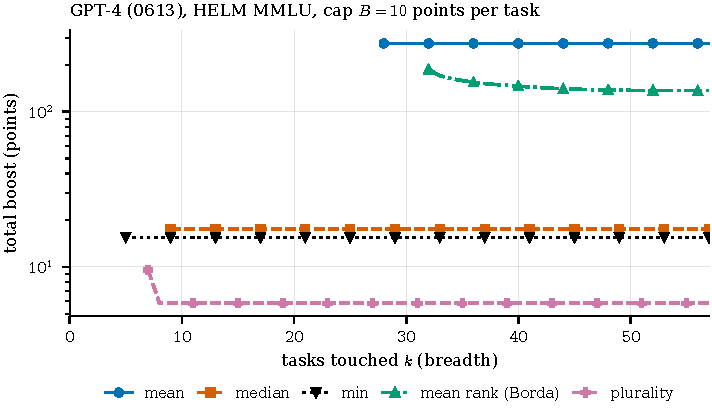
\includegraphics{../figures/fig1_teaser.pdf}
\caption{Different rules make different plans cheapest: least total boost (log scale) against tasks touched, for one target (GPT-4 0613, the one with the median range of minimal breadth across rules) on HELM MMLU at a cap of 10 points per task and each rule's own leader. The mean needs far more total boost than the median, minimum and plurality, and cannot be bought with fewer than about 28 tasks at this cap.}
\label{fig:teaser}
\end{figure}

We measure it. We define the price of first place as the breadth, depth and feasibility of the cheapest plan that puts a target model first under a rule, solve it exactly for six rule families, and compute it for the top-ranked models of three public boards: the 57 MMLU subjects of HELM and the Open LLM Leaderboard at benchmark level (six tasks) and at sub-task level (39 tasks), the latter two on the same models. We state in advance which outcomes would refute our expectations; two of them occur. Three results follow.
\begin{itemize}
\item \emph{The rules' prices differ by a factor of 7 to 19 in total boost, and the cheapest rule differs by board.} At ceilings and in the board's own points, the median over targets not yet first puts a target first on HELM for 360 points under the mean, against 36 under the median rule and 19 under plurality; on the Open LLM Leaderboard the mean needs 32 and 134 points at benchmark and sub-task level against 5 and 10 for the median rule. That the mean is dearest in points is close to an identity (its price is the sum of the deficits); the content is the size of the spread, which varies with caps and units.
\item \emph{The expected breadth ordering fails.} Median and majority rules need less breadth than the mean on HELM, the reverse of our prediction, and hold the predicted order only in part on the Open LLM Leaderboard. The dependence on the number of tasks is rule-specific and changes sign with the budget, so task granularity has no uniformly safe direction, and no rule is cheapest for 90\% of the targets on any board.
\item \emph{Cheap first place is fragile.} Holding first place with 90\% confidence under score noise costs the median rule and the minimum 3 to 7 times their noise-free depth, against 1.2 to 2 times for the mean family, on HELM and on the sub-task board.
\end{itemize}

\paragraph{Contributions.}
(i) The price of first place as a breadth--depth--feasibility triple under a boost budget, with exact solutions per rule class, computed on three public boards, with solvers checked against exhaustive search and an optimality gap reported where it is not zero (\Cref{sec:setting,sec:exact}). (ii) Pre-registered predictions reported with the verdicts as they came out: the breakdown-point intuition fails for a finite margin, and the ordering of the rules depends on the board, budget, cap and unit (\Cref{sec:breadth}). (iii) Quantities a designer can use: the budget at which the breadth ordering of two rule classes crosses, price magnitudes per rule, a within-board relation between gap and price that does not transfer across boards, and the price of confident first place under noise (\Cref{sec:pricemap,sec:predictors,sec:robustness}). A hypothesis that deficit-profile summaries predict price beyond the gap was tested and mostly failed. (iv) A calibration of the boost scale, where the conclusions hold and do not (\Cref{sec:discussion}), and a released package that prices first place on any score matrix under the seven rules studied; code and result tables are released with the paper.
